% Does Money Buy Speed? Working paper, F1 Moneyball.
% Every number in this file comes from generated/numbers.tex, built by make_assets.py
% from the datasets published on the website. To rebuild:
%   python paper/make_assets.py
%   cd paper && latexmk -pdf main.tex
\documentclass[11pt,a4paper]{article}

\usepackage[T1]{fontenc}
\usepackage[utf8]{inputenc}
\usepackage[english]{babel}
\usepackage{csquotes}
\usepackage{mathptmx}
\renewcommand{\ttdefault}{lmtt} % Latin Modern Mono: clean vector typewriter font for code and file names
\usepackage[margin=2.5cm]{geometry}
\usepackage{microtype}
\usepackage{setspace}
\usepackage{amsmath}
\usepackage{graphicx}
\usepackage{booktabs}
\usepackage{array}
\usepackage{threeparttable}
\usepackage{tabularx}
\usepackage{placeins} % \FloatBarrier keeps appendix tables in their own section
\usepackage[font=small,labelfont=bf,labelsep=period]{caption}
\usepackage[style=apa,backend=biber,natbib=true]{biblatex} % APA 7th edition
\addbibresource{references.bib}
\usepackage{xcolor}
\usepackage{fancyhdr}
\usepackage{enumitem}
\usepackage{xurl}
\usepackage[colorlinks=true,linkcolor={blue!70!black},citecolor={blue!70!black},urlcolor={blue!70!black}]{hyperref}
% Make the whole in-text citation (author and year) one link to its reference, not just the year.
\DeclareFieldFormat{citehyperref}{\DeclareFieldAlias{bibhyperref}{noformat}\bibhyperref{#1}}
\savebibmacro{cite}
\renewbibmacro*{cite}{\printtext[citehyperref]{\restorebibmacro{cite}\usebibmacro{cite}}}
\savebibmacro{textcite}
\renewbibmacro*{textcite}{\printtext[citehyperref]{\restorebibmacro{textcite}\usebibmacro{textcite}}}

% Generated by paper/make_assets.py. Do not edit by hand.
\newcommand{\AnnPwildStaff}{0.048}
\newcommand{\AnnStaff}{0.182}
\newcommand{\BootDraws}{9,999}
\newcommand{\BootSeed}{20261119}
\newcommand{\CapPStaff}{0.25}
\newcommand{\CapPwildStaff}{0.35}
\newcommand{\CapPwildTurn}{0.80}
\newcommand{\CapStaff}{0.086}
\newcommand{\CapTurn}{0.016}
\newcommand{\CiHighHeadFe}{0.100}
\newcommand{\CiHighHeadPooled}{0.147}
\newcommand{\CiHighHeadTwfe}{0.251}
\newcommand{\CiHighStaffFe}{0.084}
\newcommand{\CiHighStaffPooled}{0.126}
\newcommand{\CiHighStaffTwfe}{0.416}
\newcommand{\CiHighTurnFe}{0.053}
\newcommand{\CiHighTurnPooled}{0.112}
\newcommand{\CiHighTurnTwfe}{0.105}
\newcommand{\CiLowHeadFe}{$-$0.036}
\newcommand{\CiLowHeadPooled}{0.032}
\newcommand{\CiLowHeadTwfe}{$-$0.076}
\newcommand{\CiLowStaffFe}{$-$0.015}
\newcommand{\CiLowStaffPooled}{0.037}
\newcommand{\CiLowStaffTwfe}{$-$0.043}
\newcommand{\CiLowTurnFe}{$-$0.023}
\newcommand{\CiLowTurnPooled}{0.053}
\newcommand{\CiLowTurnTwfe}{$-$0.010}
\newcommand{\CoefHeadFe}{0.032}
\newcommand{\CoefHeadPooled}{0.090}
\newcommand{\CoefHeadTwfe}{0.088}
\newcommand{\CoefStaffFe}{0.034}
\newcommand{\CoefStaffPooled}{0.082}
\newcommand{\CoefStaffTwfe}{0.186}
\newcommand{\CoefTurnFe}{0.015}
\newcommand{\CoefTurnPooled}{0.083}
\newcommand{\CoefTurnTwfe}{0.048}
\newcommand{\CorrAll}{0.78}
\newcommand{\CorrMax}{0.98}
\newcommand{\CorrMaxYear}{2021}
\newcommand{\CorrMin}{0.50}
\newcommand{\CorrMinYear}{2014}
\newcommand{\EffCaterham}{0.00}
\newcommand{\EffEnstone}{0.68}
\newcommand{\EffManor}{0.01}
\newcommand{\EffMcLaren}{0.82}
\newcommand{\EffMercedes}{1.38}
\newcommand{\EffRedBull}{1.28}
\newcommand{\EffSilverstone}{1.07}
\newcommand{\EffWilliams}{0.41}
\newcommand{\FirstSeason}{2010}
\newcommand{\HolmN}{6}
\newcommand{\HolmPosStaff}{0.08}
\newcommand{\HolmRestMax}{0.30}
\newcommand{\HolmRestMin}{0.21}
\newcommand{\LastSeason}{2025}
\newcommand{\LooStaffcostsMax}{0.307}
\newcommand{\LooStaffcostsMin}{0.112}
\newcommand{\LooTurnoverMax}{0.070}
\newcommand{\LooTurnoverMin}{0.030}
\newcommand{\MedStaffM}{52}
\newcommand{\MedTurnM}{170}
\newcommand{\NDroppedByLag}{9}
\newcommand{\NFilings}{105}
\newcommand{\NFinFigures}{525}
\newcommand{\NObs}{95}
\newcommand{\NTeamSeasons}{104}
\newcommand{\NTeams}{8}
\newcommand{\NVerifiedChanges}{18}
\newcommand{\NoResetStaff}{0.211}
\newcommand{\OnePlaceStaff}{25}
\newcommand{\OnePlaceTurn}{94}
\newcommand{\OpsStaff}{0.129}
\newcommand{\PHeadFe}{0.36}
\newcommand{\PHeadPooled}{$<$0.01}
\newcommand{\PHeadTwfe}{0.30}
\newcommand{\PStaffFe}{0.18}
\newcommand{\PStaffPooled}{$<$0.01}
\newcommand{\PStaffTwfe}{0.11}
\newcommand{\PTurnFe}{0.44}
\newcommand{\PTurnPooled}{$<$0.01}
\newcommand{\PTurnTwfe}{0.10}
\newcommand{\PosHeadcount}{$-$3.28}
\newcommand{\PosPHeadcount}{0.04}
\newcommand{\PosPStaffcosts}{0.01}
\newcommand{\PosPTurnover}{0.02}
\newcommand{\PosPwildHeadcount}{0.046}
\newcommand{\PosPwildStaffcosts}{0.01}
\newcommand{\PosPwildTurnover}{0.06}
\newcommand{\PosStaffcosts}{$-$4.47}
\newcommand{\PosTenHeadcount}{0.31}
\newcommand{\PosTenStaffcosts}{0.43}
\newcommand{\PosTenTurnover}{0.14}
\newcommand{\PosTurnover}{$-$1.51}
\newcommand{\PpHeadFe}{0.3}
\newcommand{\PpHeadPooled}{0.9}
\newcommand{\PpHeadTwfe}{0.8}
\newcommand{\PpStaffFe}{0.3}
\newcommand{\PpStaffPooled}{0.8}
\newcommand{\PpStaffTwfe}{1.8}
\newcommand{\PpTurnFe}{0.1}
\newcommand{\PpTurnPooled}{0.8}
\newcommand{\PpTurnTwfe}{0.5}
\newcommand{\PwildHeadFe}{0.45}
\newcommand{\PwildHeadTwfe}{0.25}
\newcommand{\PwildStaffFe}{0.44}
\newcommand{\PwildStaffTwfe}{0.04}
\newcommand{\PwildTurnFe}{0.62}
\newcommand{\PwildTurnTwfe}{0.15}
\newcommand{\RealTerms}{A further check measures money in 2015 pounds with the UK consumer prices index \citep{ons_cpi}. This cannot change the two-way model, because the season effects already absorb inflation that is common to all teams. In the team-effects model the staff-cost coefficient moves from 0.034 to 0.058 (bootstrap $p = 0.40$), so the simpler models do not change in substance either. }
\newcommand{\RsqBase}{0.67}
\newcommand{\RsqOps}{0.74}
\newcommand{\SbpPwildStaff}{0.04}
\newcommand{\SbpStaff}{0.166}
\newcommand{\ScopeN}{23}
\newcommand{\ScopePStaff}{0.13}
\newcommand{\ScopePosPwildStaff}{0.02}
\newcommand{\ScopePosStaff}{$-$4.59}
\newcommand{\ScopePwildStaff}{0.11}
\newcommand{\ScopeStaff}{0.184}
\newcommand{\TenPctStaffM}{5.2}
\newcommand{\TenPctTurnM}{17}
\newcommand{\TurnAvgCaterham}{28}
\newcommand{\TurnAvgEnstone}{159}
\newcommand{\TurnAvgManor}{37}
\newcommand{\TurnAvgMcLaren}{260}
\newcommand{\TurnAvgMercedes}{325}
\newcommand{\TurnAvgRedBull}{317}
\newcommand{\TurnAvgSilverstone}{122}
\newcommand{\TurnAvgWilliams}{127}
\newcommand{\VerConstructorSeason}{47fdeadf3f5c}
\newcommand{\VerEfficiency}{f490c85abf3f}
\newcommand{\VerFinancialObservation}{c12aa42dc2bd}
\newcommand{\VerModelResults}{fb95fa8081ba}
\newcommand{\VerRobustnessChecks}{ae85825e8423}

% \input inside a tabular breaks booktabs rules; the primitive form does not.
\makeatletter\let\inputrows\@@input\makeatother

% ---------------------------------------------------------------- links to the website and code
\newcommand{\site}{https://nahianibnat-2000.github.io/F1-moneyball}
\newcommand{\repo}{https://github.com/NahianIbnat-2000/F1-moneyball}
\newcommand{\sitepage}[2]{\href{\site/#1}{#2}}
\newcommand{\code}[1]{\href{\repo/blob/main/#1}{\nolinkurl{#1}}}

\hypersetup{
  pdftitle={Does Money Buy Speed? Financial Resources and Sporting Performance in Formula 1},
  pdfauthor={Nahian Ibnat},
  pdfsubject={Working paper, November 2026},
  pdfkeywords={sports economics, Formula 1, team finances, panel data, cost cap}
}

\pagestyle{fancy}
\fancyhf{}
\renewcommand{\headrulewidth}{0pt}
\fancyfoot[C]{\footnotesize\thepage}
\fancypagestyle{plain}{\fancyhf{}\renewcommand{\headrulewidth}{0pt}%
  \fancyfoot[C]{\footnotesize\thepage}}

\setlength{\parskip}{0.35em}
\setlength{\emergencystretch}{2em} % lets long URLs in the references break without overflowing
\onehalfspacing

\title{\textbf{Does Money Buy Speed?}\\[0.3em]
  \large\textit{Financial Resources and Sporting Performance in Formula~1, \FirstSeason{} to \LastSeason}}
\author{Nahian Ibnat\thanks{Working paper, November 2026. Not peer reviewed. Part of F1 Moneyball, an independent
  Formula~1 economics and finance research platform: \url{\site/}. The interactive version of this study is at
  \url{\site/research/does-money-buy-speed}. Data and code: \url{\repo}. Project overview: \url{\site/hub/}.}}
\date{November 2026}

\begin{document}
\maketitle
\thispagestyle{plain}

\begin{abstract}
\noindent Formula~1 teams compete for a fixed set of prizes, and since 2021 a cost cap limits most of their spending. This
paper asks whether teams with more money score more points, whether a team does better in the seasons after it spends
more, and whether this link changed under the cost cap. I build a panel of audited accounts from the UK statutory filings of \NTeams{} team lineages (\NTeamSeasons{}
team-seasons, \FirstSeason{} to \LastSeason), link them to championship results, and estimate pooled and fixed-effects
models on lagged money, with inference built for a small number of teams. Between teams, money and success move together:
the correlation between turnover share and points share is \CorrAll, and 10\% more turnover in the previous season goes with
a points share about \PpTurnPooled{} percentage points higher. Within teams the evidence is weaker. The clearest result is
for staff spending: 10\% more goes with a finish about \PosTenStaffcosts{} places higher in the next season's championship
(wild cluster bootstrap $p = \PosPwildStaffcosts$). The matching points-share estimate is less certain once changes in
accounting scope are controlled for (bootstrap $p = \ScopePwildStaff$), no within-team result survives a correction for
multiple testing at the 5\% level (smallest Holm-adjusted $p = \HolmPosStaff$), and the link does not change measurably
under the cost cap. All results are associations, not causal effects. They suggest that spending on people goes with
modest gains for a team, while most of the gap between teams reflects differences that last for many years, so a spending
limit alone may narrow that gap only slowly.

\medskip\noindent\textbf{Keywords:} sports economics, competitive balance, Formula~1, team finances, panel data, cost cap.\\
\textbf{JEL codes:} Z21, Z23, L83, C23.
\end{abstract}

% ============================================================================ 1
\section{Introduction}
\label{sec:intro}

Formula~1 is a closed league of about ten teams \citep{liberty2026}, and each team is also a firm. The covered teams in this
paper had average yearly turnover between about GBP~\TurnAvgCaterham{} million (Caterham) and GBP~\TurnAvgMercedes{} million
(Mercedes) over the period studied (\hyperref[tab:desc]{Table~\ref*{tab:desc}}). Each team decides how much money to raise
and how to spend it on people, parts and facilities, and every season the championship shows how well that spending worked.
The richest teams usually finish at the front (\hyperref[fig:scatter]{Figure~\ref*{fig:scatter}}). This raises an old
question in sports economics: do the biggest spenders win because they spend more, or because the organisations that are
good at winning are also good at raising money?

The question matters for three groups. The first is the regulator. Since 2021 the
F\'ed\'eration Internationale de l'Automobile (FIA), which governs the sport, has limited how much each team may spend in a
season. This limit, the \textit{cost cap}, applies to most spending on cars and staff, but some items are left out, for
example marketing, driver pay and the pay of the team's three highest-paid staff \citep[Articles 2.3 and 3.1]{fia2021}. The
cap started at USD~145 million in 2021, fell to USD~140 million in 2022 and to USD~135 million from 2023
\citep[Article 2.3]{fia2021}. The regulations state that one aim of the cap is to promote the competitive balance of the championship, and another to
make the teams financially sustainable \citep[Article 1.3]{fia2021}. \textit{Competitive balance} is the term economists use for how close the teams in a league are to each other in strength, so that the result of a race or
season is not known in advance \citep{szymanski2003}. If money mainly buys results, a limit on money should bring the teams
closer together. If results depend more on how well a team is organised, a limit on money will do less. The second group is
team owners and investors, who need to know what extra spending can be expected to bring. The third group is researchers,
for whom Formula~1 is a clear case of firms competing for a fixed prize, with spending that is reported in audited accounts.

The difficulty is that a simple comparison of teams cannot separate the two explanations.
An \textit{association} means that two things tend to move together; a \textit{causal effect} means that changing one thing
would change the other \citep{angrist2009}. Rich teams also tend to be well run, so part of any association
between money and results may come from good management rather than from money. In addition, the link may run backwards.
Most of the sport's prize fund is paid according to results in earlier Constructors' Championships \citep{liberty2018}, so
success brings money as well as the other way round. When the outcome affects the supposed cause in this way, economists
speak of \textit{reverse causality} \citep[Chapter~16]{wooldridge2020}. This paper therefore studies associations and is careful
not to read them as causal effects.

Earlier research offers a starting point. In other sports, \citet{hall2002} test whether
a team's past payroll predicts its later results and find different answers for baseball and English football. In
Formula~1, \citet{bell2016} show that the team matters more than the driver for results, and \citet{lonik2024} find that
budget strategy is associated with better standings in the seasons from 2010 to 2020. Studies of the cost cap so far
\citep{foghsgaard2024, jung2023} ask whether the cap changed competitive balance and find no clear effect.
\hyperref[sec:lit]{Section~\ref*{sec:lit}} reviews this work in more detail.

Two things are missing from that work. To my knowledge, no study links audited financial
figures, each traced to its source, to results for the same Formula~1 teams over time, and no study separates two
different comparisons: the comparison between teams, and the comparison of each team with itself over time. The difference
matters. Comparing Mercedes with Williams in the same year asks whether richer teams do better than poorer teams. Comparing
Williams in a year when it spent more than usual with Williams in its other years asks whether a team does better when it
has more money than it normally does. The first comparison mixes money with everything else that makes Mercedes different
from Williams; the second removes those lasting differences and comes closer to the question of what extra money is
associated with. This paper makes both comparisons with the same data.

The paper asks three questions. First, do teams with more money score more
points than other teams? Second, does a team do better in the seasons after it has more money than usual? Third, has this
link changed since the cost cap was introduced? To answer them, I build a dataset of audited accounts for \NTeams{} team
lineages from \FirstSeason{} to \LastSeason, taken from the companies' public filings in the United Kingdom, and link it to
championship results. The main tool is a regression, a statistical method that estimates how much one quantity changes, on
average, when another changes \citep[Chapter~2]{wooldridge2020}. Because there are only \NTeams{} teams, the paper uses
methods for measuring uncertainty that are designed for a small number of groups.

The paper makes two contributions. First, it provides a dataset of audited financial figures for
Formula~1 teams in which every number is linked to the filing and page it came from, published so that others can reuse
and check it. Second, it separates the link between teams from the link within a team over time, uses methods suited to a
small number of teams, and extends the period studied into the cost-cap years.

Between teams, money and points go together closely (\hyperref[sec:results]{Section~\ref*{sec:results}}).
Within a team the link is much weaker. The clearest result concerns spending on staff: in the season after a team spends
10\% more on staff than it usually does, it finishes on average about \PosTenStaffcosts{} places higher in the championship.
For a team with the median staff budget in the data, GBP~\MedStaffM{} million, 10\% is about GBP~\TenPctStaffM{} million.
Put differently, finishing one place higher goes with roughly \OnePlaceStaff\% more staff spending than usual. The matching
result for a team's share of points is less certain, no within-team result passes a correction for the number of tests
made, and the link does not change measurably after the cost cap (\hyperref[sec:rob]{Section~\ref*{sec:rob}}). All of these
are associations, not causal effects.

\hyperref[sec:lit]{Section~\ref*{sec:lit}} reviews the literature.
\hyperref[sec:data]{Section~\ref*{sec:data}} describes the data and \hyperref[sec:strategy]{Section~\ref*{sec:strategy}}
the method. \hyperref[sec:results]{Section~\ref*{sec:results}} presents the results and \hyperref[sec:rob]{Section~\ref*{sec:rob}}
tests how robust they are. \hyperref[sec:discussion]{Section~\ref*{sec:discussion}} discusses what the results mean and
where they fall short, and \hyperref[sec:conclusion]{Section~\ref*{sec:conclusion}} concludes. The appendices list the data
sources, explain how the financial data were built, and show where each result comes from.

The paper is the written version of a study published on the F1 Moneyball website \citep{f1moneyball}, which shows the
same results as interactive charts and lets readers download every dataset used here
(\sitepage{research/does-money-buy-speed}{research article}; \sitepage{moneyball}{Moneyball dashboard};
\sitepage{provenance}{data provenance}; \sitepage{methodology}{methodology}). The full code is public
\citep{f1moneyballcode}, and \hyperref[app:code]{Appendix~\ref*{app:code}} maps each table and figure to the script that
produces it.

% ============================================================================ 2
\section{Literature}
\label{sec:lit}

\citet{rottenberg1956} and \citet{neale1964} explain why sports leagues need
some balance between teams. A contest whose winner is certain in advance loses its interest for spectators, so even the
strongest team gains from having strong rivals. \citet{szymanski2003} reviews how the design of a contest, including rules
on spending, shapes how much effort teams make and how outcomes are spread. This line of work is the reason regulators care
whether money decides results: if it does, limiting spending is one way to protect balance.

\citet{hall2002} ask whether higher payroll leads to better performance or
better performance leads to higher payroll. Their method is to test whether a team's spending in earlier years helps to
predict its later results. For Major League Baseball they find no evidence that payroll drives performance over their full
sample, while for English football they cannot rule it out. Their idea of testing whether past spending predicts later
results guides the design of this paper, which links each season's results to the previous season's money.

\citet{bell2016} use a statistical model that separates the contribution of
the driver from that of the team. They find that the team explains more of the results than the driver, and increasingly so
over time, which makes the team the right unit to study. \citet{jenkins2010} shows that major changes in the technical rules
can reset which teams lead, because a new set of rules can reward a different design. \citet{judde2013} study competitive
balance in Formula~1 from 1950 to 2010, including the period of the Resource Restriction Agreement, an earlier agreement
among teams to limit their resources.

The closest study is \citet{lonik2024}, who examine the seasons from 2010 to
2020, before the cost cap. Using cost-benefit analysis and regressions, they find that budget strategy is associated with
better standings, more points, more podium finishes and a higher share of races finished, and that spending on research and
development is the most effective. This paper asks a related question but differs in three ways. Its money figures come
from audited statutory accounts, each traced to its filing and page, rather than from published estimates. It separates
the link between teams from the link within a team over time, which turn out to be very different. And it extends the
period into the cost-cap years, 2021 to 2025, using methods designed for a small number of teams.

The evidence on the cost cap so far comes from student theses. \citet{foghsgaard2024} study
competitive balance from 1998 to 2023 and find no evidence that the cap increased it. They note that the 2022 technical
rules, introduced one season after the cap, make the cap's effect hard to isolate. \citet{jung2023} also finds no effect and
describes the result as preliminary. This paper does not measure competitive balance directly. Its question is narrower:
whether the link between a team's money and its results changed after 2021. Its answer, that the link did not change
measurably, is consistent with that earlier work and faces the same difficulty of separating the cap from the 2022 rules.

% ============================================================================ 3
\section{Data}
\label{sec:data}

Every company registered in the United Kingdom must prepare yearly financial statements, known
as statutory accounts, and file them at Companies House, the UK register of companies, where anyone can read them
\citep{companiesact2006,ch_register}. Eight Formula~1 team lineages are run by UK companies whose accounts cover the team:
Red Bull \citep{ch_redbull}, Mercedes \citep{ch_mercedes}, McLaren \citep{ch_mclaren}, Williams \citep{ch_williams},
Enstone, which raced as Renault, Lotus and Alpine \citep{ch_enstone}, Silverstone, which raced as Force India, Racing Point
and Aston Martin \citep{ch_forceindia,ch_amr}, Banbury, which raced as Virgin, Marussia and Manor from 2010 to 2016
\citep{ch_manor}, and Leafield, which raced as Lotus Racing and Caterham from 2010 to 2012 \citep{ch_caterham}. A
\textit{team lineage} follows one team through changes of name and owner, as long as the same company or its direct
successor runs it. \hyperref[app:sources]{Appendix~\ref*{app:sources}} gives the link to each company's filing history.
Ferrari and Racing Bulls, which are registered as Italian teams, Sauber (Swiss) and Haas (American) \citep{jolpica} are not
covered, because no UK company accounts covering the whole team were found for them on the Companies House register
\citep{ch_register}.

Three measures are taken from the accounts. \textit{Turnover} is the money a company earns from selling goods and services
in the year, after trade discounts and taxes such as value added tax \citep[s.~474]{companiesact2006}; for a racing team it
includes income such as sponsorship and prize money \citep{ch_manor}. \textit{Staff costs} are what the company spends on its
employees: wages and salaries, social security costs and pension costs \citep[s.~411(5)]{companiesact2006}.
\textit{Headcount} is the average number of people the company employed during the year, which UK companies must report
\citep[s.~411(1)]{companiesact2006}. Turnover measures the money a team has available, while staff costs and headcount
measure how much it invests in people.

Many of the older filings are scanned images rather than text, so they were read with optical character recognition (OCR),
software that turns an image of printed text into text a computer can process \citep{smith2007}. Every figure was then
checked against the previous-year column of the next filing, where companies repeat last year's figures, or against the
image of the page. Where a later filing changed (restated) a figure, the figure as first reported is used and the change is
recorded. In total the dataset holds \NFinFigures{} figures from \NFilings{} filings. Every figure, with its filing, page
and checks, can be browsed in the \sitepage{provenance}{provenance explorer}, and
\hyperref[app:construction]{Appendix~\ref*{app:construction}} explains how the dataset was built.

Results come from the Jolpica-F1 database \citep{jolpica}, which continues the widely used Ergast
database. The outcome of interest is the Constructors' Championship, the season-long ranking of teams by the points their
cars score in races. Team names change often \citep{jolpica}, so each team is followed as a lineage, as described above.

The points awarded per race have changed over time, and money rises over time
with inflation, so raw points and raw pounds are not comparable from one season to the next. The paper therefore works
with shares. A team's \textit{points share} is its points divided by the combined points of all covered teams in that
season. Its \textit{resource share} is, in the same way, its turnover (or staff costs, or headcount) divided by the total of
the covered teams. Shares are computed only in seasons where at least four covered teams report the same measure. The
\textit{efficiency ratio} divides a team's points share by its turnover share. A ratio of 1 means a team's share of the
points equals its share of the money; a ratio above 1 means it scored more than its money alone would suggest, and a ratio
below 1 means it scored less.

The data cover \NTeamSeasons{} team-seasons, where a team-season is one team in one season. The
regression models use \NObs{} of them. The difference arises because the models link each season's results to the
previous season's money, so each team's first season, and the first season after a gap in its accounts, has no previous
value to use (\NDroppedByLag{} team-seasons in all).

\hyperref[tab:desc]{Table~\ref*{tab:desc}}
summarises each team over its seasons in the data: the average turnover, staff costs and headcount, the average points
share and the average efficiency ratio. It shows three things that shape the rest of the paper. First, the teams differ
greatly in size, and these differences last: Mercedes and Red Bull had average turnover of about GBP~\TurnAvgMercedes{}
million and GBP~\TurnAvgRedBull{} million, while Williams had about GBP~\TurnAvgWilliams{} million. Differences that last
for many years are exactly what the within-team comparison is designed to remove. Second, money is not the whole story:
Silverstone, with average turnover of about GBP~\TurnAvgSilverstone{} million, had an efficiency ratio of
\EffSilverstone, scoring slightly more than its share of the money, while McLaren, with about GBP~\TurnAvgMcLaren{}
million, had a ratio of \EffMcLaren. Third, the two smallest teams, Manor and Caterham, scored almost no points, and their
accounts are incomplete, as the table notes explain, so their figures understate their full budgets.

\begin{table}[htbp]
\centering
\begin{threeparttable}
\caption{Covered teams, averages over their seasons}
\label{tab:desc}
\small
\begin{tabular}{@{}p{4.2cm}lrrrrr@{}}
\toprule
Team lineage & Seasons & \multicolumn{1}{c}{Turnover} & \multicolumn{1}{c}{Staff costs} & \multicolumn{1}{c}{Staff} & \multicolumn{1}{c}{Points} & \multicolumn{1}{c}{Efficiency} \\
 & (count) & \multicolumn{1}{c}{(GBP m)} & \multicolumn{1}{c}{(GBP m)} & \multicolumn{1}{c}{(people)} & \multicolumn{1}{c}{share (\%)} & \multicolumn{1}{c}{ratio} \\
\midrule
\inputrows generated/table1_descriptives.tex 
\bottomrule
\end{tabular}
\begin{tablenotes}[flushleft]\footnotesize
\item \textit{Notes:} \NTeamSeasons{} team-seasons. Money in nominal GBP, not adjusted for inflation. Points share and
efficiency ratio are computed among the covered teams in each season. Manor and Caterham accounts are partial: in 2010 Manor did no research and
development itself but hired outside technical expertise, and bought the business of Wirth Technologies in 2011
\citep{ch_manor}; Caterham's UK company provided design, testing and race-support services to its Malaysian parent company
\citep{ch_caterham}. Their figures therefore understate the full team budget. \textit{Source:} datasets \texttt{financial\_observation} (version \VerFinancialObservation)
and \texttt{efficiency} (version \VerEfficiency), \sitepage{data}{F1 Moneyball data explorer}.
\end{tablenotes}
\end{threeparttable}
\end{table}

% ============================================================================ 4
\section{Empirical strategy}
\label{sec:strategy}

The main model is a linear regression of a team's points share on the logarithm of one of its
resources in the previous season:
\begin{equation}
  \text{PointsShare}_{it} = \beta \log(\text{Resource}_{i,t-1}) + \alpha_i + \gamma_t + \varepsilon_{it},
  \label{eq:main}
\end{equation}
where $i$ is a team lineage and $t$ a season. The coefficient $\beta$ is the quantity of interest. It measures how much
points share changes, on average, when the resource changes. The resource enters as a logarithm, which means that $\beta$
describes the link with a \textit{percentage} change in money rather than a change in pounds: for a small change, a change
of 0.1 in the logarithm is close to a 10\% change in the resource \citep[Chapter~6]{wooldridge2020}. This suits the data,
because GBP~10 million is a large increase for Manor but a small one for Mercedes, while 10\% means the same for both.
Because points share is measured from 0 to 1, $\beta \times \log(1.1) \times 100$ gives the change in percentage points of
points share that goes with 10\% more of the resource. The term $\varepsilon_{it}$ collects everything else that affects
results and is not in the model.

Resources enter with a one-season lag: this season's points are linked to
last season's money. As explained in the introduction, success brings prize money \citep{liberty2018}, so money and points
measured in the same season would partly reflect points causing money. Using last season's money reduces this problem but
does not remove it, because a team that is improving may attract both more money and more points over several seasons.

The data form a \textit{panel}, meaning the same teams are observed in many
seasons \citep[Chapter~10]{wooldridge2010}. A panel allows three versions of equation~(\ref{eq:main}), and each answers a different question.

The first version, the \textit{pooled} model, leaves out $\alpha_i$ and $\gamma_t$. It treats every team-season as a
separate observation and compares them all with each other, so it asks whether richer teams score more points than poorer
teams. This is the comparison shown in \hyperref[fig:scatter]{Figure~\ref*{fig:scatter}}.

The second version adds $\alpha_i$, a separate constant for each team, known as a \textit{team fixed effect}. A fixed effect
captures everything about a team that stays the same over time, such as its factory, its culture or its long-run reputation
\citep[Chapter~14]{wooldridge2020}. Once these constants are in the model, each team is compared only with its own average,
so the model asks whether a team does better in the seasons after it had more money than it usually has. Lasting
differences between teams, which drive the pooled comparison, no longer play a role.

The third version, the \textit{two-way fixed-effects} model, adds $\gamma_t$, a separate constant for each season, as well.
A season effect captures everything that affects all teams in the same season, such as a new set of technical rules or
general inflation \citep[Chapter~5]{angrist2009}. This model compares a team with its own average and, at the same time,
with the other teams in the same season.

The two-way model is the main within-team test, for a specific reason. Points shares add up to one in every season, so
they cannot rise for all teams at once. Money in pounds, by contrast, rises for most teams over time
(\hyperref[tab:desc]{Table~\ref*{tab:desc}}), partly through general inflation \citep{ons_cpi}. Without season effects,
this common rise in spending has no matching rise in points, which pulls the estimated link towards zero. Season effects
remove the common rise and leave each team's spending relative to the other teams in that season.

Every estimate comes with a measure of how uncertain it is. A \textit{95\% confidence
interval} is a range built so that, if the study were repeated many times, 95\% of such ranges would contain the true value
\citep[Chapter~4]{wooldridge2020}. A \textit{p-value} is the probability of finding a link at least as strong as the one
observed if in fact there were no link at all; a small p-value means the observed link would be unusual if there were no
true link, but it does not measure how large or important the link is \citep{wasserstein2016}. By convention, a p-value
below 0.05 is called statistically significant.

Uncertainty is measured with standard errors \textit{clustered} by team. Clustering allows for the fact that a team's
results in different seasons are related to each other, so that sixteen seasons of the same team carry less independent
information than sixteen different teams \citep{cameron2015}. Clustered standard errors work well when there are many
groups, but with only \NTeams{} teams they can understate the uncertainty \citep{cameron2008}. The within-team estimates
therefore also get a p-value from a \textit{wild cluster bootstrap}. A bootstrap estimates uncertainty by building many
artificial versions of the data from the data itself and re-estimating the model on each one; the wild cluster version
does this by changing the sign and size of each team's errors together, which keeps the link between a team's seasons
\citep{cameron2008}. This paper uses the restricted version with Webb's six-point weights and \BootDraws{} draws, which
behaves better than the usual weights when there are very few groups \citep{webb2023}. None of these methods turns an
association into a causal effect; all results describe how money and results move together.

% ============================================================================ 5
\section{Results}
\label{sec:results}

\hyperref[fig:scatter]{Figure~\ref*{fig:scatter}} shows the basic pattern in the data. Each
point is one team in one season. The horizontal position is the team's share of turnover and the vertical position its
share of points. The dashed line marks equal shares, so a point above the line is a team-season that scored more than its
share of the money, and a point below it scored less. The points rise clearly from left to right: teams with a larger share
of the money usually have a larger share of the points. The correlation, a number between $-1$ and $1$ that measures how
closely two quantities move together in a straight line \citep[Appendix~B]{wooldridge2020}, is \CorrAll{} over all
\NTeamSeasons{} team-seasons. In single seasons it ranges from \CorrMin{} (\CorrMinYear) to \CorrMax{} (\CorrMaxYear). The
figure matters because it shows how strong the link between teams is before any model is applied. It also shows that teams
with similar money can end up far apart, which is what the efficiency ratio measures: over the whole period, Mercedes
(efficiency ratio \EffMercedes) and Red Bull (\EffRedBull) turned their money into points far more effectively than
Williams (\EffWilliams), Manor (\EffManor) or Caterham (\EffCaterham). The same chart, with filters by team and season, is
on the \sitepage{moneyball}{Moneyball dashboard}.

\begin{figure}[htbp]
\centering
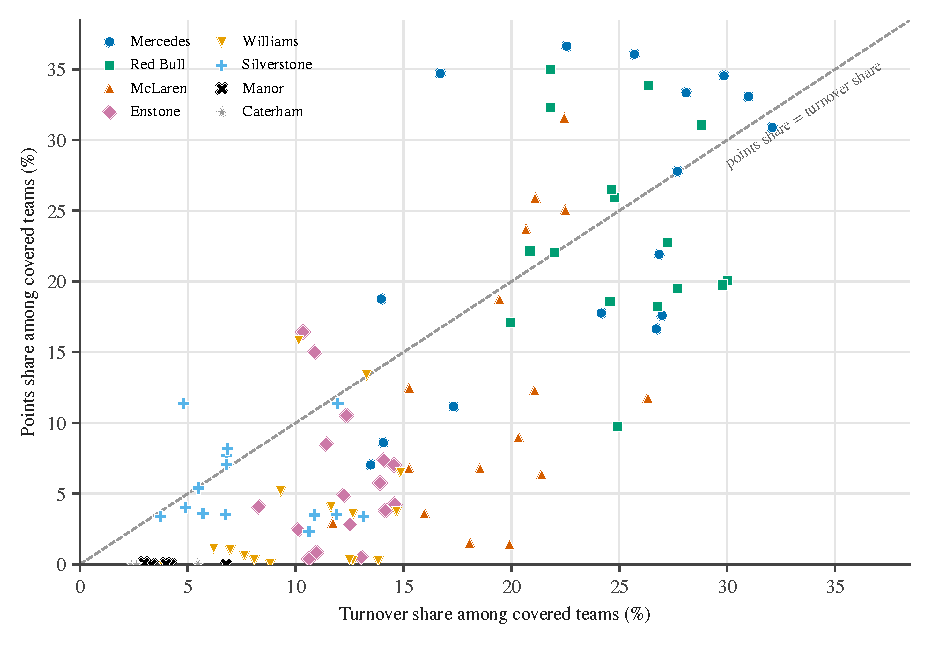
\includegraphics[width=0.9\textwidth]{generated/fig1_scatter.pdf}
\caption{Turnover share and points share by team-season, \FirstSeason{} to \LastSeason. Each point is one team in one
season; the dashed line marks equal shares, so points above it scored more than their share of money. \textit{Source:}
dataset \texttt{efficiency}; interactive version on the \sitepage{moneyball}{Moneyball dashboard}.}
\label{fig:scatter}
\end{figure}

\hyperref[tab:models]{Table~\ref*{tab:models}}
reports the three versions of the model for each of the three resources. Each row gives the coefficient $\beta$, its 95\%
confidence interval, two p-values (clustered, and from the wild bootstrap for the within-team models), the number of
team-seasons used ($N$) and the number of teams. \hyperref[fig:coef]{Figure~\ref*{fig:coef}} shows the same coefficients
and confidence intervals as a chart. The figure matters because it makes the key pattern visible at a glance: the pooled
estimates are precise and clearly above zero, while the within-team intervals are wide and all of them cross zero, which
means the data cannot rule out that there is no within-team link at all.

In the pooled model, the turnover coefficient is \CoefTurnPooled{}
(95\% confidence interval \CiLowTurnPooled{} to \CiHighTurnPooled). In economic terms, a team with 10\% more turnover than
another team in the previous season has, on average, a points share about \PpTurnPooled{} percentage points higher. For a
team with the median turnover in the data, GBP~\MedTurnM{} million, 10\% is about GBP~\TenPctTurnM{} million.
The confidence interval lies well above zero, so the link between teams is clear. Staff costs (\CoefStaffPooled) and
headcount (\CoefHeadPooled) give similar results.

When each team is compared only with its own average,
the turnover coefficient falls to \CoefTurnFe{} (clustered $p = \PTurnFe$, bootstrap $p = \PwildTurnFe$), much smaller than
the pooled value and no longer distinguishable from zero. This is the most important pattern in the table. It
means that most of the pooled link comes from lasting differences between teams, not from a team doing better in the
seasons when it had more money than usual. The richest teams are also the teams that win year after year, but a given
team's results move only a little with its own changes in money.

Adding season effects raises the estimates, as the
explanation in \hyperref[sec:strategy]{Section~\ref*{sec:strategy}} leads one to expect. For turnover the coefficient is
\CoefTurnTwfe{} (clustered $p = \PTurnTwfe$). The largest within-team estimate is for staff costs, \CoefStaffTwfe. In
economic terms, a team that spends 10\% more on staff than usual, relative to the other teams that season, has a points
share about \PpStaffTwfe{} percentage points higher in the next season. Its clustered p-value is \PStaffTwfe{} and its
bootstrap p-value \PwildStaffTwfe. The two methods fall on different sides of the 0.05 convention and the confidence
interval (\CiLowStaffTwfe{} to \CiHighStaffTwfe) includes zero, so this estimate alone is not strong evidence. As
\hyperref[sec:rob]{Section~\ref*{sec:rob}} shows, it also becomes less certain when changes in the way accounts are drawn up
are taken into account, while the same pattern with championship position as the outcome holds up better.

\begin{table}[htbp]
\centering
\begin{threeparttable}
\caption{Points share on log resources in the previous season}
\label{tab:models}
\small
\begin{tabular}{@{}llrcrrrr@{}}
\toprule
Measure & Model & Coef. & 95\% CI & $p$ (clustered) & $p$ (bootstrap) & $N$ & Teams \\
\midrule
\inputrows generated/table2_models.tex 
\bottomrule
\end{tabular}
\begin{tablenotes}[flushleft]\footnotesize
\item \textit{Notes:} OLS estimates of \hyperref[eq:main]{equation~(\ref*{eq:main})}. Standard errors clustered by team. Bootstrap: wild cluster
restricted bootstrap, Webb six-point weights, 9,999 draws, within-team models only. \textit{Source:} datasets
\texttt{model\_results} (version \VerModelResults) and \texttt{robustness\_checks} (version \VerRobustnessChecks); code in
\code{src/f1moneyball/econometrics/models.py}.
\end{tablenotes}
\end{threeparttable}
\end{table}

\begin{figure}[htbp]
\centering
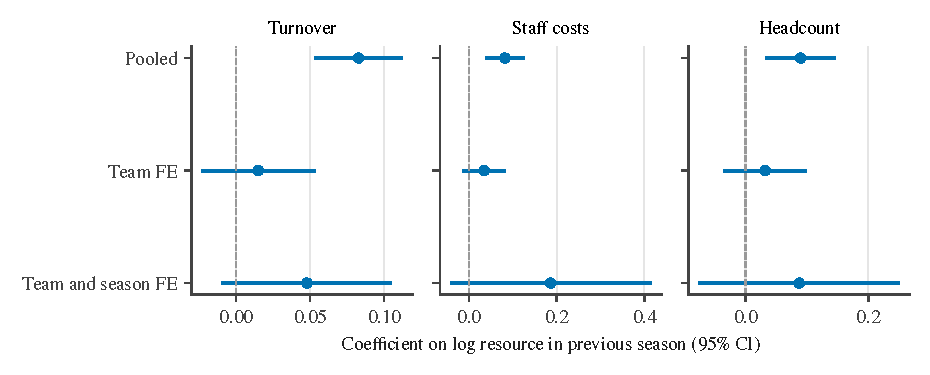
\includegraphics[width=\textwidth]{generated/fig2_coefficients.pdf}
\caption{Coefficients and 95\% confidence intervals from \hyperref[tab:models]{Table~\ref*{tab:models}}. The dashed line marks zero.}
\label{fig:coef}
\end{figure}

% ============================================================================ 6
\section{Robustness}
\label{sec:rob}

A result is \textit{robust} if it stays similar when reasonable choices in the analysis are made differently. Robustness
checks matter because a result that depends on one particular choice, one season or one team is a weak basis for any
conclusion. \hyperref[tab:rob]{Table~\ref*{tab:rob}} collects the main checks. All use the two-way model, and the last
column repeats the main result from \hyperref[tab:models]{Table~\ref*{tab:models}} so that each check can be compared with
it.

Large changes in the technical rules can reshuffle the order of teams for reasons unrelated to
money \citep{jenkins2010}. Leaving out the three seasons with the largest rule changes (2014, 2017 and 2022;
\citealp{fia2014tech,fia2017tech,fia2022tech}) barely changes the estimates: the staff-cost coefficient is
\NoResetStaff{} instead of \CoefStaffTwfe.

With only \NTeams{} teams, a single team could drive the results. Re-estimating the model
\NTeams{} times, each time leaving out one team, shows that the size of the within-team estimates moves a lot but the
direction never changes: the staff-cost coefficient ranges from \LooStaffcostsMin{} to \LooStaffcostsMax, and the turnover
coefficient from \LooTurnoverMin{} to \LooTurnoverMax.

Points share depends on the scoring rules, so the model is also estimated
with the team's position in the Constructors' Championship as the outcome, where a lower number is better. All three
resources go with a better position the next season: turnover \PosTurnover{} places per unit of the logarithm (clustered
$p = \PosPTurnover$, bootstrap $p = \PosPwildTurnover$), staff costs \PosStaffcosts{} ($p = \PosPStaffcosts$, bootstrap
$p = \PosPwildStaffcosts$) and headcount \PosHeadcount{} ($p = \PosPHeadcount$, bootstrap $p = \PosPwildHeadcount$). In
economic terms, a team that spends 10\% more on staff than usual finishes, on average, about \PosTenStaffcosts{} places
higher in the next season's championship. For a team with the median staff budget of about GBP~\MedStaffM{} million, 10\%
is about GBP~\TenPctStaffM{} million. Put the other way round, one place higher goes with about \OnePlaceStaff\% more staff
spending than usual, and with about \OnePlaceTurn\% more turnover. Here the two methods for measuring uncertainty give
similar p-values. This is the clearest within-team result in the paper, but it is still an association: a team that is
improving may hire more staff and finish higher for the same underlying reason.

To test whether the link changed after the cap, the model adds an \textit{interaction}: a term
that lets the coefficient on money take a different value from 2021 onward \citep[Chapter~7]{wooldridge2020}. For staff
costs the change is \CapStaff{} (clustered $p = \CapPStaff$, bootstrap $p = \CapPwildStaff$), and for turnover \CapTurn{}
(bootstrap $p = \CapPwildTurn$). Neither is distinguishable from zero, so the link does not change measurably under the
cost cap. With only five cap seasons, and the 2022 rules arriving one season after the cap, this test can detect only a
large change.

Adding the share of races a team finishes and the average number of places it gains from
its starting position raises the share of the variation in points explained by the model, the \textit{R-squared}
\citep[Chapter~3]{wooldridge2020}, from \RsqBase{} to \RsqOps, and reduces the staff-cost coefficient to \OpsStaff. Part of the link between staff spending and points therefore
shows up in reliability and race-day performance. These two
measures come from the same season as the outcome, however, and may themselves be results of spending, so this check is
read as a description of where the link shows up rather than as a separate test.

The accounts are not all drawn up in the same way, and three checks test whether
this matters. First, some teams file \textit{group accounts}, which combine the parent company with the companies it
controls (its subsidiaries) into one set of figures \citep[s.~404]{companiesact2006}, while others file accounts for one
company alone. Four teams switch between the two during the period (\hyperref[tab:scope]{Table~\ref*{tab:scope}}), so a
change in their figures may partly reflect a change in what is counted. Adding an indicator for group accounts in the
previous season (\ScopeN{} team-seasons) leaves the staff-cost coefficient almost unchanged (\ScopeStaff{} against
\CoefStaffTwfe), but its bootstrap p-value rises from \PwildStaffTwfe{} to \ScopePwildStaff. With championship position as
the outcome, the staff-cost estimate keeps its size (\ScopePosStaff{} places per unit of the logarithm) and its bootstrap
p-value stays at \ScopePosPwildStaff. Second, a few accounting periods are longer or shorter than a year
(\hyperref[tab:periods]{Table~\ref*{tab:periods}}); scaling turnover and staff costs to 365 days gives a staff-cost
coefficient of \AnnStaff{} (bootstrap $p = \AnnPwildStaff$). Third, McLaren's staff costs for 2023 to 2025 include large
\textit{share-based payments}, that is, pay in the form of shares or amounts linked to the value of shares
\citep{ifrs2,ch_mclaren}; removing them gives \SbpStaff{} (bootstrap $p = \SbpPwildStaff$). \RealTerms These checks show
that the points-share result is most sensitive to the type of accounts, while the position result is the steadier of the
two.

The main model is estimated for three resources and two outcomes, which makes six
within-team tests. The more tests are made, the more likely it is that one of them gives a small p-value by chance alone.
The Holm method adjusts the p-values for this by requiring the smallest p-value to pass a stricter threshold, the next
smallest a slightly less strict one, and so on \citep{holm1979}. After this adjustment, the smallest p-value is
\HolmPosStaff{} (staff costs and championship position) and the others lie between \HolmRestMin{} and \HolmRestMax. No
within-team result is statistically significant at the 5\% level after the correction. The staff-cost result for position
comes closest, which is why the paper describes it as suggestive rather than established.

Read as a whole, the table shows which parts of the
result can be relied on. The direction of the within-team link, more money going with better results, survives every
check. Its size is uncertain, the points-share result depends on how the accounts are drawn up, and the position result for
staff spending is the most stable. Every estimate behind the table, including each run that leaves out one team, is listed
on the \sitepage{research/does-money-buy-speed}{research article page}.

\begin{table}[htbp]
\centering
\begin{threeparttable}
\caption{Robustness checks (team and season fixed effects)}
\label{tab:rob}
\small
\begin{tabular}{@{}>{\raggedright\arraybackslash}p{4.6cm}lccc@{}}
\toprule
Check & Measure & Coefficient & $p$ (clustered, bootstrap) & Main result \\
\midrule
\inputrows generated/table3_robustness.tex 
\bottomrule
\end{tabular}
\begin{tablenotes}[flushleft]\footnotesize
\item \textit{Notes:} ``Main result'' is the team and season fixed-effects coefficient from \hyperref[tab:models]{Table~\ref*{tab:models}}.
Clustered $p$-values; wild bootstrap $p$-values in parentheses where computed. The two accounting-scope rows add an
indicator for group-consolidated accounts in the previous year.
$^{a}$~Coefficient on log resource $\times$ cost-cap period (2021 onward).
$^{b}$~Places in the championship per log point of the resource; negative means a better position.
$^{c}$~Share-based payments removed where the filing amount is recorded (McLaren 2023 to 2025).
\textit{Source:} dataset \texttt{robustness\_checks} (version \VerRobustnessChecks); code in
\code{src/f1moneyball/econometrics/robustness.py}.
\end{tablenotes}
\end{threeparttable}
\end{table}

% ============================================================================ 7
\section{Discussion and limitations}
\label{sec:discussion}

Between teams, money and points go together: the richest teams win most
(\hyperref[fig:scatter]{Figure~\ref*{fig:scatter}}). Within teams, the picture depends on how the comparison is made.
Comparing a team only with its own average shows no clear link (\hyperref[tab:models]{Table~\ref*{tab:models}}). Comparing
it with its own average and with the other teams in the same season, more money, and staff spending in particular, comes
before better results in the next season, in both points share and championship position
(\hyperref[tab:models]{Tables~\ref*{tab:models}} and~\hyperref[tab:rob]{\ref*{tab:rob}}). The direction is the same in every
check, but the size is uncertain, the evidence rests on \NTeams{} teams, the points-share result weakens when the type of
accounts is controlled for, and no single within-team test survives the correction for multiple testing. The fairest
reading is that extra spending, especially on people, goes with modest improvements within a team, while most of the gap
between teams reflects differences that last for many years. This fits a picture in which money and success build up
together over time, since most of the prize fund is paid according to earlier championship results \citep{liberty2018}.

Several limitations should be kept in mind. The most important is the small number of teams.
Eight teams give little information for the within-team comparison, which limits how precise the estimates can be, and the
methods used to measure uncertainty can only partly make up for this \citep{cameron2015}.

A second limitation is that the accounts belong to legal companies rather than to teams. A company's accounts may include
business that has nothing to do with racing, or leave out costs that are held elsewhere in a group. The clearest examples
are Manor, which in 2010 bought in its engineering from outside \citep{ch_manor}, and Caterham, whose UK company provided
services to a Malaysian parent company \citep{ch_caterham}. Related to this, accounting periods, accounting standards and
the type of accounts (group or company) differ across teams and years. The checks in
\hyperref[sec:rob]{Section~\ref*{sec:rob}} address these differences only in part.

A third limitation is reverse causality. Because success brings prize money, a team's results may drive its spending as
well as the other way round. Linking results to the previous season's money reduces this problem but cannot remove it, so
none of the results can be read as the effect of spending more.

A fourth limitation concerns inflation and coverage. Money is measured in pounds of each year. The two-way model removes
general inflation through the season effects, and the simpler models are checked in 2015 pounds in
\hyperref[sec:rob]{Section~\ref*{sec:rob}}, but other price changes specific to Formula~1 are not captured. The data also
leave out Ferrari and the other non-UK teams, so the results describe the UK-based teams only.

Finally, the cost cap and the 2022 technical rules arrived one season apart \citep{fia2021,fia2022tech}. With data measured
once per season, their effects cannot be separated, so the finding of no change under the cap should be read as
preliminary.

% ============================================================================ 8
\section{Conclusion}
\label{sec:conclusion}

This paper asked whether Formula~1 teams with more money do better, using the audited accounts of \NTeams{} team lineages
from \FirstSeason{} to \LastSeason. The main findings answer its three questions. Between teams, money and success go
together closely: the teams that spend the most score the most points, with a correlation of \CorrAll{} between turnover
share and points share (\hyperref[sec:results]{Section~\ref*{sec:results}}). Within a team, the link is weaker. The
clearest result is that a team spending 10\% more on staff than usual finishes about \PosTenStaffcosts{} places higher in
the next season's championship, while the same link with points share is less certain and no within-team result passes a
correction for multiple testing at the 5\% level (\hyperref[sec:results]{Sections~\ref*{sec:results}}
and~\hyperref[sec:rob]{\ref*{sec:rob}}). The link does not change measurably under the cost cap
(\hyperref[tab:rob]{Table~\ref*{tab:rob}}).

These findings fit together. If money alone decided results, the link within a team would be as strong as the link between
teams. Instead, most of the gap between teams reflects differences that last for many years, which may include
organisation, facilities and experience, and extra spending goes with only modest gains for a given team. That staff
spending shows the clearest link suggests that money matters most when it is spent on people.

Three criticisms are reasonable. First, success may cause spending rather than the other way round, since most of the prize
fund is paid according to earlier results \citep{liberty2018}. The one-season lag reduces this problem but does not remove
it, so the results are associations, not causal effects. Second, the accounts belong to legal companies and are not all
drawn up in the same way. The checks in \hyperref[sec:rob]{Section~\ref*{sec:rob}} show that the position result holds when
changes in the type of accounts are controlled for, while the points-share result weakens. Third, eight teams is a small
sample. The wild cluster bootstrap and the Holm correction take this into account, which is why the within-team results are
described as suggestive. \hyperref[sec:discussion]{Section~\ref*{sec:discussion}} sets out the remaining limitations.

The findings agree with earlier work. They match \citet{lonik2024}, who find that budget strategy is associated with better
standings, and \citet{bell2016}, who find that the team explains much of the results. \citet{hall2002} test whether past
payroll predicts later results and find mixed evidence across sports; here too, the link from past spending to later
results within a team is weaker and less certain than the link between teams. And like \citet{foghsgaard2024} and
\citet{jung2023}, this paper finds no clear change under the cost cap so far, with the same difficulty of separating the cap
from the 2022 technical rules.

For empirical work, the main value of this study is a dataset that anyone can check: every figure is linked to its filing
and page, and all data and code are public. For policy, the results suggest that a cost cap may narrow the gap between
teams only slowly, because much of that gap does not depend on current spending. Future research could add Ferrari and the
non-UK teams, use more seasons under the cost cap, split spending by purpose, and look for changes in rules or prize money
that change a team's budget for reasons unrelated to its results, which would allow a closer test of cause and effect.

% ============================================================================ data + code
\section*{Data and code availability}
\addcontentsline{toc}{section}{Data and code availability}

All data, code and the data dictionary are public. The website \url{\site/} shows every dataset with its sources and a
download link, and the GitHub repository \url{\repo} holds the pipeline, the econometrics and the source of this paper
(folder \code{paper}). The figures in this paper come from these dataset versions:
\texttt{financial\_observation} \VerFinancialObservation; \texttt{efficiency} \VerEfficiency;
\texttt{model\_results} \VerModelResults; \texttt{robustness\_checks} \VerRobustnessChecks;
\texttt{constructor\_season} \VerConstructorSeason. The website shows the current version of each dataset on its
\sitepage{data}{data page}, so a reader can check whether the data have changed since this paper was written.

\clearpage
% Centred "References" heading, kept in the PDF bookmarks.
\defbibheading{centred}{\phantomsection\addcontentsline{toc}{section}{References}%
  \begin{center}{\Large\bfseries References}\end{center}\vspace{0.3em}}
\setlength{\bibitemsep}{0.9\baselineskip}   % blank line between references
\setlength{\bibhang}{1.5em}                 % hanging indent for second and later lines
\setcounter{biburlnumpenalty}{9000}          % break long links after / or - rather than inside words
\setcounter{biburllcpenalty}{9000}
\setcounter{biburlucpenalty}{9000}
\printbibliography[heading=centred]

% ============================================================================ appendix
\clearpage
\appendix
\begin{center}
  {\Large\bfseries Appendix}
\end{center}
\addcontentsline{toc}{section}{Appendix}
\vspace{0.5em}
\section{Data sources}
\label{app:sources}

\noindent Every figure in this paper comes from one of the public sources below. Each link opens the page the data were
collected from (accessed 19 November 2026). The same links are stored next to every figure in the published datasets
(column \texttt{source\_url}) and shown in the \sitepage{data}{data explorer}.

\begin{table}[htbp]
\centering
\footnotesize
\renewcommand{\arraystretch}{1.25}
\begin{tabularx}{\textwidth}{@{}>{\raggedright\arraybackslash}p{3.6cm}>{\raggedright\arraybackslash}p{3.4cm}>{\raggedright\arraybackslash}X@{}}
\toprule
Data & Source & Link \\
\midrule
Mercedes accounts & \citet{ch_mercedes} & \url{https://find-and-update.company-information.service.gov.uk/company/00787446/filing-history} \\
Red Bull accounts & \citet{ch_redbull} & \url{https://find-and-update.company-information.service.gov.uk/company/05202976/filing-history} \\
McLaren accounts & \citet{ch_mclaren} & \url{https://find-and-update.company-information.service.gov.uk/company/01517478/filing-history} \\
Williams accounts & \citet{ch_williams} & \url{https://find-and-update.company-information.service.gov.uk/company/01297497/filing-history} \\
Enstone accounts (Renault, Lotus, Alpine) & \citet{ch_enstone} & \url{https://find-and-update.company-information.service.gov.uk/company/01806337/filing-history} \\
Silverstone accounts, 2010--2016 (Force India) & \citet{ch_forceindia} & \url{https://find-and-update.company-information.service.gov.uk/company/02417588/filing-history} \\
Silverstone accounts, 2019--2025 (Racing Point, Aston Martin) & \citet{ch_amr} & \url{https://find-and-update.company-information.service.gov.uk/company/11496673/filing-history} \\
Banbury accounts (Virgin, Marussia, Manor) & \citet{ch_manor} & \url{https://find-and-update.company-information.service.gov.uk/company/06661964/filing-history} \\
Leafield accounts (Lotus Racing, Caterham) & \citet{ch_caterham} & \url{https://find-and-update.company-information.service.gov.uk/company/07042086/filing-history} \\
\addlinespace
Race results, championship standings & \citet{jolpica} & \url{https://api.jolpi.ca/ergast/f1/} \\
Cost cap levels & \citet{fia2021} & \url{https://www.fia.com/sites/default/files/formula_1_-_financial_regulations_-_2021_-_iss_8_-_2021-10-15.pdf} \\
\bottomrule
\end{tabularx}
\end{table}

\FloatBarrier
\section{How the financial data were built}
\label{app:construction}

\noindent The financial dataset holds \NFinFigures{} figures from \NFilings{} audited filings. Each figure is stored with its
company, registration number, accounting period, the page of the filing it was read from, any change made to it, and a link
to the filing. A copy of every filing is kept in the repository (folder \code{data/source_documents}), so each figure can be
checked even if the online register changes. The \sitepage{provenance}{provenance explorer} shows all of this for every team
and season.

Five rules were used to build the data. First, a team is followed through changes of name and owner
when the same UK company, or its direct successor, keeps running it (\hyperref[app:sources]{Appendix~\ref*{app:sources}}
lists the companies). Second, each accounting period is mapped to the season it mostly covers; for a year ending in
December this is the same calendar year, and periods that cover only a few months between two full years are kept in the
data but not mapped to a season. Third, money is recorded in full pounds, so amounts reported in thousands are multiplied by
1,000, and headcount is the average monthly number of employees as reported \citep[s.~411(3)]{companiesact2006}; all
amounts are nominal, that is, in pounds of each year. Fourth, when a later filing restates a figure, the figure as first
reported is used and the restatement is recorded in the notes. Fifth, where no full-year accounts exist, as for Force India
in 2017 and 2018, during and after its administration \citep{ch_forceindia}, the team-season is recorded as missing rather
than filled in.

\hyperref[tab:periods]{Table~\ref*{tab:periods}} lists the filings that do not cover about twelve months. They are used
as reported in the main models; the check in \hyperref[sec:rob]{Section~\ref*{sec:rob}} scales them to 365 days.

\begin{table}[htbp]
\centering
\begin{threeparttable}
\caption{Accounting periods that do not cover about twelve months}
\label{tab:periods}
\footnotesize
\begin{tabularx}{\textwidth}{@{}>{\raggedright\arraybackslash}p{3.6cm}>{\raggedright\arraybackslash}Xlrl@{}}
\toprule
Team lineage & Company & Period & Days & Season \\
\midrule
\inputrows generated/tableC1_periods.tex 
\bottomrule
\end{tabularx}
\begin{tablenotes}[flushleft]\footnotesize
\item \textit{Source:} dataset \texttt{financial\_observation} (version \VerFinancialObservation).
\end{tablenotes}
\end{threeparttable}
\end{table}

Some companies file group accounts, which include their subsidiaries, and others file
accounts for the company alone. Four teams switch between the two during the sample (\hyperref[tab:scope]{Table~\ref*{tab:scope}}), so a change in
their figures can partly reflect what the accounts include. \hyperref[sec:rob]{Section~\ref*{sec:rob}} controls for this.

\begin{table}[htbp]
\centering
\begin{threeparttable}
\caption{Seasons with company and group accounts}
\label{tab:scope}
\footnotesize
\begin{tabularx}{\textwidth}{@{}>{\raggedright\arraybackslash}Xll@{}}
\toprule
Team lineage & Company accounts & Group accounts \\
\midrule
\inputrows generated/tableC2_scope.tex 
\bottomrule
\end{tabularx}
\begin{tablenotes}[flushleft]\footnotesize
\item \textit{Source:} dataset \texttt{financial\_observation}, turnover rows (version \VerFinancialObservation).
\end{tablenotes}
\end{threeparttable}
\end{table}

Automated checks run every time the data are rebuilt: plausible ranges, one figure per team, season and
measure, accounting periods, changes in accounting scope, and year-on-year changes above 50\%. Each of the
\NVerifiedChanges{} large year-on-year changes in turnover or staff costs was checked against the saved filings by reading
the stated page for both years; all matched. The record of this check is \code{data/manual/verified_large_changes.csv}, and
the script that repeats it is \code{scripts/verify_large_changes.py}.

\FloatBarrier
\section{Where each result comes from}
\label{app:code}

\noindent To reproduce the paper from scratch:
\begin{verbatim}
git clone https://github.com/NahianIbnat-2000/F1-moneyball.git
cd F1-moneyball
pip install -e .
python -m f1moneyball.pipeline all     # download, build, estimate, publish
python paper/make_assets.py            # numbers, tables, figures
cd paper && latexmk -pdf main.tex      # this paper
\end{verbatim}
\noindent The published results were produced by the repository's GitHub Actions workflows with Python 3.12. For exact
package versions, install from \code{requirements-lock.txt} instead. The wild cluster bootstrap uses \BootDraws{} draws
with a fixed random seed (\BootSeed), so it gives the same $p$-values on every run.

\begin{table}[htbp]
\centering
\small
\begin{tabularx}{\textwidth}{@{}lX@{}}
\toprule
Paper element & Code (links open the file on GitHub) \\
\midrule
Financial figures & \code{data/manual/financial_observations.csv}; entry rules in \code{docs/MANUAL_FINANCIAL_ENTRY.md} \\
Race results, standings & \code{src/f1moneyball/ingestion/jolpica.py} \\
Shares, efficiency ratio & \code{src/f1moneyball/econometrics/efficiency.py} \\
\hyperref[tab:models]{Table~\ref*{tab:models}}, \hyperref[fig:coef]{Figure~\ref*{fig:coef}} & \code{src/f1moneyball/econometrics/models.py} \\
\hyperref[tab:rob]{Table~\ref*{tab:rob}}, bootstrap & \code{src/f1moneyball/econometrics/robustness.py} \\
Pipeline steps & \code{src/f1moneyball/pipeline.py} \\
Data checks & \code{src/f1moneyball/validation/checks.py}; \code{scripts/verify_large_changes.py} \\
All numbers, tables, figures here & \code{paper/make_assets.py} \\
This document & \code{paper/main.tex}, \code{paper/references.bib} \\
\bottomrule
\end{tabularx}
\end{table}

\end{document}
